\documentclass{article}

%
% 引入模板的style文件
%
\usepackage{homework}

\setCJKmainfont{SimSun}[AutoFakeBold] %宋体加粗
\setCJKsansfont{SimHei}[AutoFakeBold] %黑体加粗


\usepackage{minted} %配合minted宏包进行好看的高亮
\usepackage{currfile} %配合minted宏包进行好看的高亮
\usepackage{caption} %配合minted宏包进行好看的高亮
\usepackage{tcolorbox} %配合minted宏包进行好看的高亮
\usepackage{xcolor} %配合minted宏包进行好看的高亮
\tcbuselibrary{skins} %配合minted宏包进行好看的高亮
\tcbuselibrary{minted} %配合minted宏包进行好看的高亮
\usemintedstyle{paraiso-dark} %配合minted宏包进行好看的高亮



%
% 封面
%

\title{
	
\includegraphics[width=0.6\textwidth]{images/title/ucas_logo 1.pdf}\\
    \vspace{1in}
    \textmd{\textbf{\hmwkClass}}\\
	\textmd{\Large{\textbf{\hmwkClassID}}}\\
    \textmd{\textbf{\hmwkTitle}}\\
    \normalsize\vspace{0.1in}\large{\hmwkCompleteTime }\\
    \vspace{0.1in}\large{\textit{\hmwkClassInstructor\ }}\\
    \vspace{1in}
	
\includegraphics[width=0.25\textwidth]{images/title/Cyber.jpg}\\
	\vspace{1in}
}


\author{
	\hmwkAuthorName \\ 
	\hmwkAuthorStuID \\
	\hmwkAuthorInst \\
	\hmwkAuthorzhuanye \\
	\hmwkAuthorfangxiang
	}
\date{}

\renewcommand{\part}[1]{\textbf{\large Part \Alph{partCounter}}\stepcounter{partCounter}\\}


%
% 正文部分
%
\begin{document}


\maketitle


%\include{chapters/ch01}
%\include{chapters/ch02}
%\include{chapters/ch03}
%\include{chapters/ch04}
%\include{chapters/ch05}


\pagebreak

\begin{homeworkProblem}
	在一个10类的模式识别问题中, 有3类单独满足多类情况1, 其余的类别满足多类情况2. 问该模式识别问题所需判别函数的最少数目是多少?
	\\

	\solution 将10类问题可看作4类满足多类情况1的问题, 可将3类单独满足多类情况1的类找出来, 剩下的7类全部划到4类中剩下的一个子类中. 再在此子类中, 运用多类情况2的判别法则进行分类, 此时需要$7\ast (7-1)/2=21$个判别函数. 故共需要4+21=25个判别函数.
\end{homeworkProblem}

\begin{homeworkProblem}
	一个三类问题, 其判别函数如下:
	$$d_1\left( \boldsymbol{x} \right) =-x_1,\,\, d_2\left( \boldsymbol{x} \right) =x_1+x_2-1,\,\, d_3\left( \boldsymbol{x} \right) =x_1-x_2-1
	$$

	(1). 设这些函数是在多类情况1条件下确定的,绘出其判别界面和每一个模式类别的区域.

	(2). 设为多类情况2, 并使: $d_{12}\left( \boldsymbol{x} \right) =d_1\left( \boldsymbol{x} \right) , d_{13}\left( \boldsymbol{x} \right) =d_2\left( \boldsymbol{x} \right) , d_{23}\left( \boldsymbol{x} \right) =d_3\left( \boldsymbol{x} \right)$. 绘出其判别界面和多类情况2的区域.

	(3). 设$d_1\left( \boldsymbol{x} \right) ,d_2\left( \boldsymbol{x} \right)$和$d_3\left( \boldsymbol{x} \right)$是在多类情况3的条件下确定的, 绘出其判别界面和每类的区域.
	\\

	\solution 三种情况分别如下图\ref{fig:判别界面与区域}中所示:

	\begin{figure}[H]  % 这里记得用[H]
		\centering
		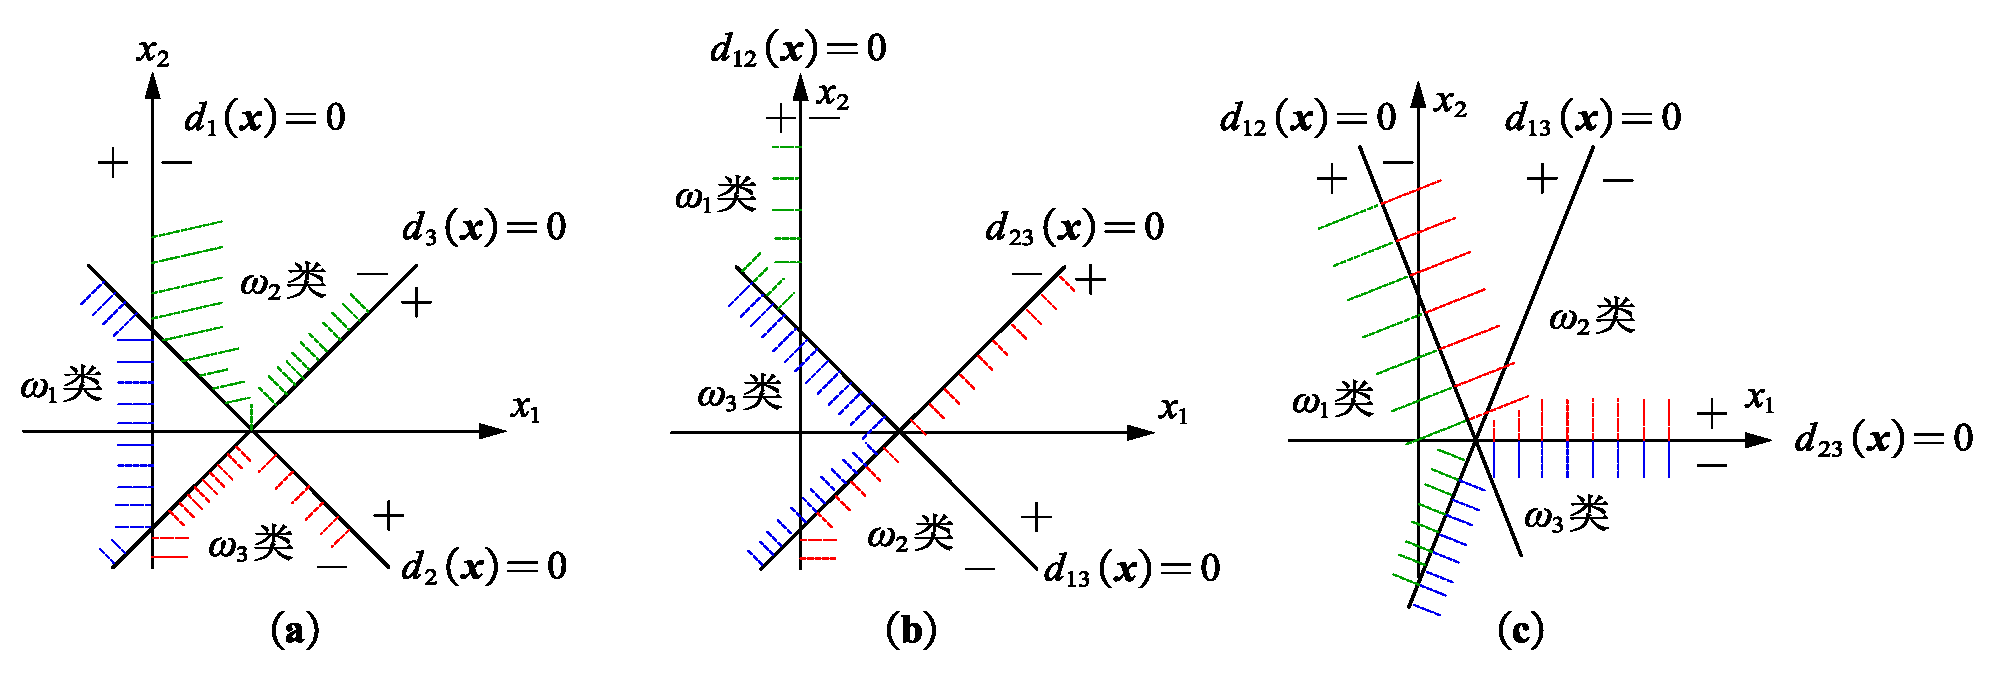
\includegraphics[width=1.0\textwidth]{images/title/判别界面与区域.pdf}
		\caption{判别界面与区域}
		\label{fig:判别界面与区域}
	\end{figure}
\end{homeworkProblem}

\begin{homeworkProblem}
	两类模式, 每类包括5个3维不同的模式, 且良好分布. 如果它们是线性可分的, 问权向量至少需要几个系数分量? 假如要建立二次的多项式判别函数, 又至少需要几个系数分量? (设模式的良好分布不因模式变化而改变)
	\\

	\solution \,\,(1). 若是线性可分的, 则权向量需要至少$n+1=4$个系数分量;

	(2). 根据公式易知此情形下的系数分量个数至少为$\displaystyle N_{\omega}=C_{n+r}^{r}=\frac{\left( n+r \right) !}{r!n!}=\frac{5!}{2!3!}=10	$.
\end{homeworkProblem}

\pagebreak

\begin{homeworkProblem}
	1. 用感知器算法求下列模式分类的解向量$\boldsymbol{w}$:
	\begin{align}
		\omega _1&=\left\{ \left( 0,0,0 \right) ^{\mathrm{T}},\left( 1,0,0 \right) ^{\mathrm{T}},\left( 1,0,1 \right) ^{\mathrm{T}},\left( 1,1,0 \right) ^{\mathrm{T}} \right\} \notag
		\\
		\omega _2&=\left\{ \left( 0,0,1 \right) ^{\mathrm{T}},\left( 0,1,1 \right) ^{\mathrm{T}},\left( 0,1,0 \right) ^{\mathrm{T}},\left( 1,1,1 \right) ^{\mathrm{T}} \right\} \notag
	\end{align}
	
	\solution 将属于$\omega_2$的训练样本乘以$(-1)$, 并写成增广向量的形式:
	\begin{align}
		x_1&=\left( 0,0,0,1 \right) ^{\mathrm{T}}, x_2=\left( 1,0,0,1 \right) ^{\mathrm{T}}, x_3=\left( 1,0,1,1 \right) ^{\mathrm{T}}, x_4=\left( 1,1,0,1 \right) ^{\mathrm{T}} \notag
		\\
		x_5&=\left( 0,0,-1,-1 \right) ^{\mathrm{T}}, x_6=\left( 0,-1,-1,-1 \right) ^{\mathrm{T}}, x_7=\left( 0,-1,0,-1 \right) ^{\mathrm{T}}, x_8=\left( -1,-1,-1,-1 \right) ^{\mathrm{T}} \notag
	\end{align}
	迭代选取$C=1,w_1=(0,0,0,0)^{\mathrm{T}}$, 则迭代过程中权向量变换如下:
	\begin{align}
		w\left( 2 \right) &=\left( 0,0,0,1 \right) ^{\mathrm{T}}, w\left( 3 \right) =\left( 0,0,-1,0 \right) , w\left( 4 \right) =\left( 0,-1,-1,-1 \right) ^{\mathrm{T}}, w\left( 5 \right) =\left( 0,-1,-1,0 \right) ^{\mathrm{T}} \notag
		\\
		w\left( 6 \right) &=\left( 1,-1,-1,1 \right) ^{\mathrm{T}}, w\left( 7 \right) =\left( 1,-1,-2,0 \right) ^{\mathrm{T}}, w\left( 8 \right) =\left( 1,-1,-2,1 \right) ^{\mathrm{T}}, w\left( 9 \right) =\left( 2,-1,-1,2 \right) ^{\mathrm{T}} \notag
		\\
		w\left( 10 \right) &=\left( 2,-1,-2,1 \right) ^{\mathrm{T}}, w\left( 11 \right) =\left( 2,-2,-2,0 \right) ^{\mathrm{T}}, w\left( 12 \right) =\left( 2,-2,-2,1 \right) ^{\mathrm{T}}\left( \text{此时已收敛} \right) \notag 
	\end{align}
	所以最终得到解向量$\boldsymbol{w}=(2,-2,-2,1)^{\mathrm{T}}$, 相应的判别函数为$d(\boldsymbol{x})=2x_1-2x_2-2x_3+1$.
	\\

	2. 编写求解上述问题的感知器算法程序.
	\\

	\solution \,\,C++代码如下:
\begin{tcblisting}{listing engine=minted,boxrule=0.1mm,
colback=blue!5!white,colframe=blue!75!black,
listing only,left=5mm,enhanced,sharp corners=all,
overlay={\begin{tcbclipinterior}\fill[red!20!blue!20!white] (frame.south west)
rectangle ([xshift=5mm]frame.north west);\end{tcbclipinterior}},
minted language=c++,
minted style=tango,
minted options={fontsize=\small,breaklines,autogobble,linenos,numbersep=3mm}}
#include <iostream>
#include <algorithm>
#include <vector>
#include <numeric>
using namespace std;

int main() {
    int d, n1, n2, C;
    cout << "请依次输入样本维数d, w1类的样本数n1, w2类的样本数n2, 迭代步长C" << endl;
    cin >> d >> n1 >> n2 >> C;
    vector<vector<float>> omega_1(n1, vector<float>(d));
    vector<vector<float>> omega_2(n2, vector<float>(d));
    cout << "请依次输入w1类的模式样本" << endl;
    for(int i = 0; i < n1; i++) {
        for(int j = 0; j < d; j++) {
            cout << " omega_1[" << i << "][" << j << "] : ";
            cin >> omega_1[i][j];
        }
    }
    cout << "请依次输入w2类的模式样本" << endl;
    for(int i = 0; i < n2; i++) {
        for(int j = 0; j < d; j++) {
            cout << " omega_2[" << i << "][" << j << "] : ";
            cin >> omega_2[i][j];
        }
    }

\end{tcblisting}

\begin{tcblisting}{listing engine=minted,boxrule=0.1mm,
colback=blue!5!white,colframe=blue!75!black,
listing only,left=5mm,enhanced,sharp corners=all,
overlay={\begin{tcbclipinterior}\fill[red!20!blue!20!white] (frame.south west)
rectangle ([xshift=5mm]frame.north west);\end{tcbclipinterior}},
minted language=c++,
minted style=tango,
minted options={fontsize=\small,breaklines,autogobble,linenos,numbersep=3mm}}
    vector<vector<float>> sample_1(n1, vector<float>(d + 1));
    vector<vector<float>> sample_2(n2, vector<float>(d + 1));
    /*增广后的w1类的模式样本*/
    for(int i = 0; i < n1; i++) {
        copy(omega_1[i].begin(), omega_1[i].end(), sample_1[i].begin());
        sample_1[i][d] = 1;
    }
    /*增广后的w2类的模式样本*/
    for(int i = 0; i < n2; i++) {
        copy(omega_2[i].begin(), omega_2[i].end(), sample_2[i].begin());
        sample_2[i][d] = 1;
    }
    for(int i = 0; i < n2; i++) {
        for(int j = 0; j < d + 1; j++) {
            sample_2[i][j] = (-1.0) * sample_2[i][j];  //增广的w2训练样本乘以-1
        }
    }
    int n = n1 + n2;
    vector<vector<float>> sample(n, vector<float>(d + 1));
    copy(sample_1.begin(), sample_1.end(), sample.begin());
    copy(sample_2.begin(), sample_2.end(), sample.begin() + n1);
    vector<float> w(d + 1, 0);
    int cnt = 0;
    while (cnt != n) { //当被正确分类的样本数cnt等于总样本数n时, 结束循环
        cnt = 0; //计数变量清零
        for(int i = 0; i < n; i++) {
            if(inner_product(w.begin(), w.end(), sample[i].begin(), 0.0) > 0) {
                cnt++;  //若被正确分类, 则权向量不变且对应的样本数自增一
            }
            else {
                for(int j = 0; j < d + 1; j++) {  //若x(k)被错误分类,
                    w[j] = w[j] + C * sample[i][j];  //则w(k+1) = w(k) + C * x(k)
                }
            }
        }
    }
    cout << "解向量w的分量分别为" << endl;
    for(int i = 0; i < d + 1; i++) {
        cout << " w[" << i << "]"  << " = " << w[i];
    }
    return 0;
}
\end{tcblisting}

程序执行结果如下图\ref{fig:程序运行结果}所示:
\begin{figure}[H]  % 这里记得用[H]
	\centering
	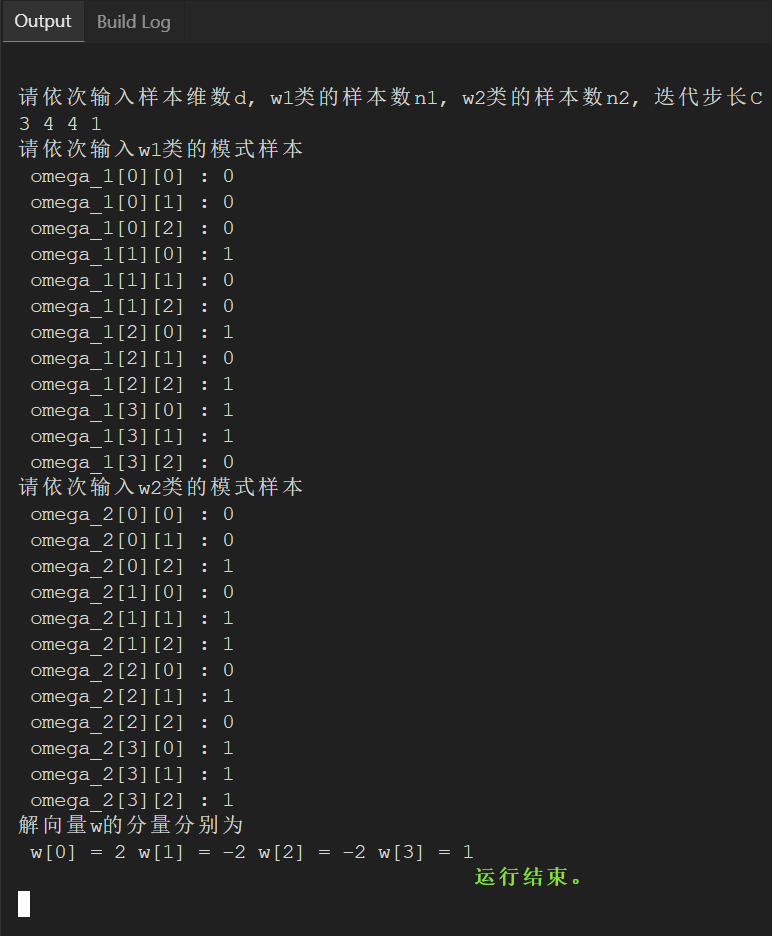
\includegraphics[width=0.8\textwidth]{images/title/P4运行结果.png}
	\caption{Problem 4 程序运行结果}
	\label{fig:程序运行结果}
\end{figure}
\end{homeworkProblem}

\pagebreak

\begin{homeworkProblem}
	用多类感知器算法求下列模式的判别函数:
	$$\omega _1:\left( -1,-1 \right) ^{\mathrm{T}},  \omega _2:\left( 0,0 \right) ^{\mathrm{T}},  \omega _3:\left( 1,1 \right) ^{\mathrm{T}}
	$$

	\solution 采用一般化的感知器算法, 将模式样本写成增广形式, 即
	$$x_1=\left( -1,-1,1 \right) ^{\mathrm{T}}, x_2=\left( 0,0,1 \right) ^{\mathrm{T}}, x_3=\left( 1,1,1 \right) ^{\mathrm{T}}
	$$
	取初始值$w_1=w_2=w_3=(0,0,0)^{\mathrm{T}}$, 取$C=1$. 
	
	以$x_1$为训练样本来进行第一次迭代, 计算内积得到$d_1(1)=d_2(1)=d_3(1)=0$, 故
	$$w_1\left( 2 \right) =\left( -1,-1,1 \right) ^{\mathrm{T}}, w_2\left( 2 \right) =\left( 1,1,-1 \right) ^{\mathrm{T}}, w_3\left( 2 \right) =\left( 1,1,-1 \right) ^{\mathrm{T}}
	$$

	以$x_2$为训练样本来进行第2次迭代, 计算内积得到$d_1(2)=1,d_2(2)=-1,d_3(2)=-1$, 故$$w_1\left( 3 \right) =\left( -1,-1,0 \right) ^{\mathrm{T}}, w_2\left( 3 \right) =\left( 1,1,0 \right) ^{\mathrm{T}}, w_3\left( 3 \right) =\left( 1,1,-2 \right) ^{\mathrm{T}}
	$$

	以$x_3$为训练样本来进行第3次迭代, 计算内积得到$d_1(3)=-2, d_2(3)=2, d_3(3)=0$, 故$$w_1\left( 4 \right) =\left( -1,-1,0 \right) ^{\mathrm{T}}, w_2\left( 4 \right) =\left( 0,0,-1 \right) ^{\mathrm{T}}, w_3\left( 4 \right) =\left( 2,2,-1 \right) ^{\mathrm{T}}
	$$

	以$x_1$为训练样本来进行第4次迭代, 计算内积得到$d_1(4)=2,d_2(4)=-1,d_3(4)=-5$, 显然$x_1$被正确分类了, 故权向量此时不用更新;

	以$x_2$为训练样本来进行第5次迭代, 计算内积得到$d_1(5)=0, d_2(5)=-1, d_3(5)=-1$, 故
	$$w_1\left( 6 \right) =\left( -1,-1,-1 \right) ^{\mathrm{T}}, w_2\left( 6 \right) =\left( 0,0,0 \right) ^{\mathrm{T}}, w_3\left( 6 \right) =\left( 2,2,-2 \right) ^{\mathrm{T}}
	$$

	以$x_3$为训练样本来进行第6次迭代, 计算内积得到$d_1(6)=-3, d_2(6)=0, d_3(6)=2$, 显然$x_3$被正确分类了, 故权向量此时不用更新;

	以$x_1$为训练样本来进行第7次迭代, 计算内积得到$d_1(7)=1, d_2(7)=0, d_3(7)=-6$, 显然$x_1$被正确分类了, 故权向量此时不用更新;

	以$x_2$为训练样本来进行第8次迭代, 计算内积得到$d_1(8)=-1, d_2(8)=0, d_3(8)=-2$, 显然$x_2$被正确分类了, 故权向量此时不用更新. 由于第6,7,8次迭代中对$x_1,x_2,x_3$均以正确分类, 故权向量的解为$w_1=\left( -1,-1,-1 \right) ^{\mathrm{T}},w_2=\left( 0,0,0 \right) ^{\mathrm{T}},w_3=\left( 2,2,-2 \right) ^{\mathrm{T}}$且判别函数为$d_1\left( \boldsymbol{x} \right) =-x_1-x_2-1, d_2\left( \boldsymbol{x} \right) =0, d_3\left( \boldsymbol{x} \right) =2x_1+2x_2-2$. 类似Problem4, 可以编写出多类感知器算法的C++程序(见后页), 程序执行结果如下图\ref{fig:P5程序运行结果}中所示:
	\begin{figure}[H]  % 这里记得用[H]
		\centering
		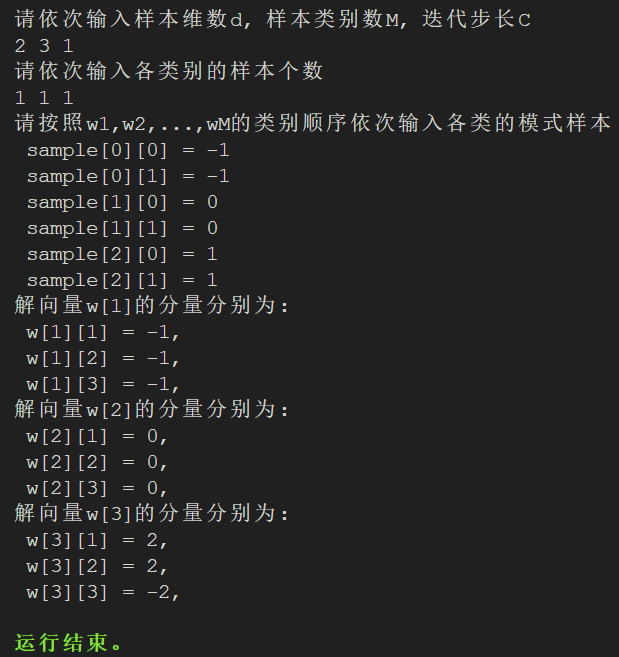
\includegraphics[width=0.4\textwidth]{images/title/作业题5-代码结果.png}
		\caption{Problem 5 程序运行结果}
		\label{fig:P5程序运行结果}
	\end{figure}
\begin{tcblisting}{listing engine=minted,boxrule=0.1mm,
colback=blue!5!white,colframe=blue!75!black,
listing only,left=5mm,enhanced,sharp corners=all,
overlay={\begin{tcbclipinterior}\fill[red!20!blue!20!white] (frame.south west)
rectangle ([xshift=5mm]frame.north west);\end{tcbclipinterior}},
minted language=c++,
minted style=tango,
minted options={fontsize=\small,breaklines,autogobble,linenos,numbersep=3mm}}
#include <iostream>
#include <algorithm>
#include <vector>
#include <numeric>
using namespace std;

int main() {
    int d, M, C;
    cout << "请依次输入样本维数d, 样本类别数M, 迭代步长C" << endl;
    cin >> d >> M >> C;
    vector<int> N(M);

    cout << "请依次输入各类别的样本个数" << endl;
    for(int i = 0; i < M; i++) {
        cin >> N[i];
    }

    int n = accumulate(N.begin(), N.end(), 0);
    vector<vector<float>> sample_init(n, vector<float>(d));
    cout << "请按照w1,w2,...,wM的类别顺序依次输入各类的模式样本" << endl;
    for(int i = 0; i < n; i++) {
        for(int j = 0; j < d; j++) {
            cout << " sample[" << i << "][" << j << "] = ";
            cin >> sample_init[i][j];
        }
    }
    
    vector<vector<float>> sample(n, vector<float>(d + 1));
    for(int i = 0; i < n; i++) {
        copy(sample_init[i].begin(), sample_init[i].end(), sample[i].begin());
        sample[i][d] = 1;
    }
    vector<vector<float>> w(M, vector<float>(d + 1, 0));
    vector<float> D(M);
    int cnt = 0;
    while (cnt != n) { //当被正确分类的样本数cnt等于总样本数n时, 结束循环
        cnt = 0; //每一轮迭代都需要把计数变量cnt清零
        for(int i = 0; i < n; i++) {
            for(int m = 0; m < M; m++) {
                D[m] = inner_product(w[m].begin(), w[m].end(), sample[i].begin(), 0.0);
            }
            int index = max_element(D.begin(), D.end()) - D.begin();
            int flag = count(D.begin(), D.end(), D[index]);
            if(i <= N[0] - 1 && i >= 0) { //第1类需要单独判断, 否则会越界
                if(index + 1 == 1 && flag == 1) {
                    cnt++;  //若当前样本被正确分类, 则权向量不变且对应的样本数自增一
                }
                else {  //若当前样本没被正确分类, 则按算法规则调整权向量
                    for(int m = 0; m < M; m++) {
                        if(D[m] >= D[0] && m != 0) {
                            for(int j = 0; j < d + 1; j++) {
                                w[m][j] = w[m][j] - C * sample[i][j];
                            }
                        }
\end{tcblisting}
\begin{tcblisting}{listing engine=minted,boxrule=0.1mm,
colback=blue!5!white,colframe=blue!75!black,
listing only,left=5mm,enhanced,sharp corners=all,
overlay={\begin{tcbclipinterior}\fill[red!20!blue!20!white] (frame.south west)
rectangle ([xshift=5mm]frame.north west);\end{tcbclipinterior}},
minted language=c++,
minted style=tango,
minted options={fontsize=\small,breaklines,autogobble,linenos,numbersep=3mm}}
                        else if(D[m] < D[0]) {
                            ;
                        }
                        else if(m == 0) {
                            for(int j = 0; j < d + 1; j++) {
                                w[m][j] = w[m][j] + C * sample[i][j];
                            }
                        }
                    }
                }
            }
            else {
                int Class = 2;
                for(int k = 2; k <= M; k++) {
                    int left = accumulate(N.begin(), N.begin() + k - 1, 0);
                    int right = accumulate(N.begin(), N.begin() + k, 0) - 1;
                    if(i >= left && i <= right) {
                        Class = k;  //求出当前样本所在的真实类别(即第k类)
                        break;
                    }
                }

                if(index + 1 == Class && flag == 1) { 
                    cnt++;  //若当前样本被正确分类, 则权向量不变且对应的样本数自增一
                }

                else {  //若当前样本没被正确分类, 则按规则调整权向量
                    for(int m = 0; m < M; m++) {
                        if(D[m] >= D[Class - 1] && m != Class - 1) {
                            for(int j = 0; j < d + 1; j++) {
                                w[m][j] = w[m][j] - C * sample[i][j];
                            }
                        }
                        else if(D[m] < D[Class - 1]) {
                            ;
                        }
                        else if(m == Class - 1) {
                            for(int j = 0; j < d + 1; j++) {
                                w[m][j] = w[m][j] + C * sample[i][j];
                            }
                        }
                    }
                }
            }
        }
    }
    for(int i = 0; i < M; i++) {
        cout << "解向量w[" << i + 1 << "]的分量分别为: " << endl;
        for(int j = 0; j < d + 1; j++) {
            cout << " w[" << i + 1 << "][" << j + 1 << "] = " << w[i][j] << "," << endl;
        }
    }
    return 0;
}
\end{tcblisting}
\end{homeworkProblem}


\pagebreak

\begin{homeworkProblem}
	采用梯度法和准则函数$\displaystyle J\left( w,x,b \right) =\frac{1}{8\left\| x \right\| ^2}\left[ \left( w^{\mathrm{T}}x-b \right) -\left| w^{\mathrm{T}}x-b \right| \right] ^2$(其中$b>0$), 试导出两类模式的分类算法.
	\\

	\solution 上述式子对$w$求导可得$$\frac{\partial J}{\partial w}=\frac{1}{4\left\| x \right\| ^2}\left[ \left( w^{\mathrm{T}}x-b \right) -\left| w^{\mathrm{T}}x-b \right| \right] \cdot \left[ x-x\cdot \mathrm{sgn} \left( w^{\mathrm{T}}x-b \right) \right] 
	$$
	其中$\mathrm{sgn}$表示符号函数, 即$\mathrm{sgn} \left( w^{\mathrm{T}}x-b \right) =\begin{cases}
		1,w^{\mathrm{T}}x-b>0\\
		-1,w^{\mathrm{T}}x-b\le 0\\
	\end{cases}$.

	于是可得到迭代式$$w\left( k+1 \right) =w\left( k \right) +C\frac{\partial J}{\partial w\left( k \right)}=w\left( k \right) +\begin{cases}
		0, w^{\mathrm{T}}\left( k \right) x-b>0\\
		\frac{w^{\mathrm{T}}\left( k \right) x-b}{\left\| x \right\| ^2}Cx, w^{\mathrm{T}}\left( k \right) x-b\le 0\\
	\end{cases}
	$$

	\vspace{3cm}

	至此, Chap 3的作业解答完毕.

	\vspace{3cm}

	\begin{figure}[H]  % 这里记得用[H]
		\centering
		
\includegraphics[width=0.6\linewidth]{images/title/ucas_logo 1.pdf}
		%\caption{ucas-logo}
		\label{fig:ucas-logo}
	\end{figure}
\end{homeworkProblem}


\pagebreak







% 引用文献
%\bibliographystyle{unsrt}  % unsrt:根据引用顺序编号
%\bibliography{refs}


\end{document}
